\chapter{Meging and Maxing\label{chap:megmax}}
Mysterious energies power temporary and persistent changes of form.
Dynamax and Gigantamax forms operate on the scale of attacks.
Mega and Primal forms are assumed for hours.
Fused and Crowned forms persist until explicitly undone.
\autoref{chap:speciesbytype} has instructions for interpreting form cards.

\section{Dynamax and Gigantamax forms\label{sec:dmaxgmax}}
Pokémon capable of Dynamax or Gigantamax form can participate in Max Battles (\autoref{sec:maxbattles}).
They can be acquired through Research, by winning Max Battles, and via trade.
These forms have access to three Max Moves: Max Attack, Max Guard, and Max Spirit.
Max Moves have four levels: Locked, 1, 2, and 3.
A freshly acquired Dynamax or Gigantamax Pokémon has Max Attack at level 1, while Max Guard and Max Spirit are both locked.
Unlocking and upgrading moves costs Max Particles and Candy of the Pokémon's genus (\autoref{table:maxupgrades});
 the amount of Candy depends on the Pokémon's cost group (\autoref{sec:costgroups}).
There are eighteen Max Attacks, one for each type, and the Max Attack known by a Dynamax Pokémon matches its fast attack.
Gigantamax Pokémon instead know a species-specific G-Max attack which cannot change.
Max Move levels persist across evolution and use of Fast TMs.
Max Attacks of level 1, 2, and 3 have power 250, 300, and 350
  respectively.
G-Max attacks have power of 350, 400, and 450, 100 more than Dynamax attacks of the same level.
Max Guard bestows a protective shield (the Guard) on all active Pokémon
  with fewer than three Guards.
This Guard will absorb 20, 40, or 60 points of damage, depending on Max Guard's level.
Max Spirit restores HP to active Pokémon.
The amount restored is a percentage of each affected Pokémon's MHP\@;
  the percentage (8\%, 10\%, or 12\%) is based on Max Spirit's level.
\begin{table}
\centering
\begin{tabular}{lrrr}
Level & Max Particles & Candy & Candy XL\\
\Midrule
1 (Unlock) & 400 & 50--80 &\\
2          & 600 & 100--130 &\\
3          & 800 & & 40--55\\
\end{tabular}
\caption{Upgrade costs for Dynamax and Gigantamax moves\label{table:maxupgrades}}
\end{table}

\input{out/dynas}
\input{out/gigantas}
\section{Mega and Primal forms\label{sec:mega}\label{sec:primal}}
\nopagecolor
Mega Evolution and Primal Reversion are almost equivalent; where I write Mega,
 read ``Mega (evolution) or Primal (reversion)'' unless otherwise noted.
Species with corresponding Mega or Primal Energy (no species has both) can take on the relevant form for eight hours.
Only one of a Trainer's Pokémon can be in its Mega form at any given time---Mega
  evolving Pokémon will cause any existing Mega forms to revert.
Mega evolution revives and fully heals the evolved Pokémon, and persists across
  fainting (i.e. the evolved Pokémon can be revived into the Mega form).
Fainting does not stop the eight hour counter.
When the evolution expires, the Pokémon has a rest period before it can Mega evolve again.
Mega Pokémon cannot be used in Max Battles, cannot defend gyms, and cannot be traded while in Mega form.
The first evolution of a Pokémon per calendar day counts towards its Mega level,
  which affects the cost to evolve, the downtime, and bonuses (\autoref{table:megalevels}).
Mega levels are reset upon a trade.
When actively battling in a raid, Mega Pokémon provide a 30\% boost to attacks of aligned
  type by \textit{other Trainers' Pokémon}, and 10\% to unaligned attacks,
  \textit{except for} Mega Rayquaza and Primal forms, which provide the boost just
  by being in the raiding party (i.e.\ they needn't be active)\footnote{Just
  for fun, Mega Rayquaza provides this bonus to Psychic attacks in addition to
  Flying and Dragon. Don't blame me, man; I didn't do it.}.
This boost is never applied to the Trainer's own Pokémon, and they do not stack.
\begin{table}
\centering
\begin{tabular}{lrrrp{.4\textwidth}}
Level & Evols & Rest days & Cost & Bonuses\\
\Midrule
0 &  0 & 14 & 100\% & 1 Candy\\
1 &  1 &  7 & 20\% & 1 Candy\\
2 &  7 &  5 & 10\% & 1 Candy\newline{}10\% Candy XL chance\newline{}50 XP\\
3 & 30 &  3 &  5\% & 2 Candy\newline{}25\% Candy XL chance\newline{}100 XP\\
\end{tabular}
\caption{Mega evolution and Primal reversion levels\label{table:megalevels}}
\end{table}
\input{out/mega}
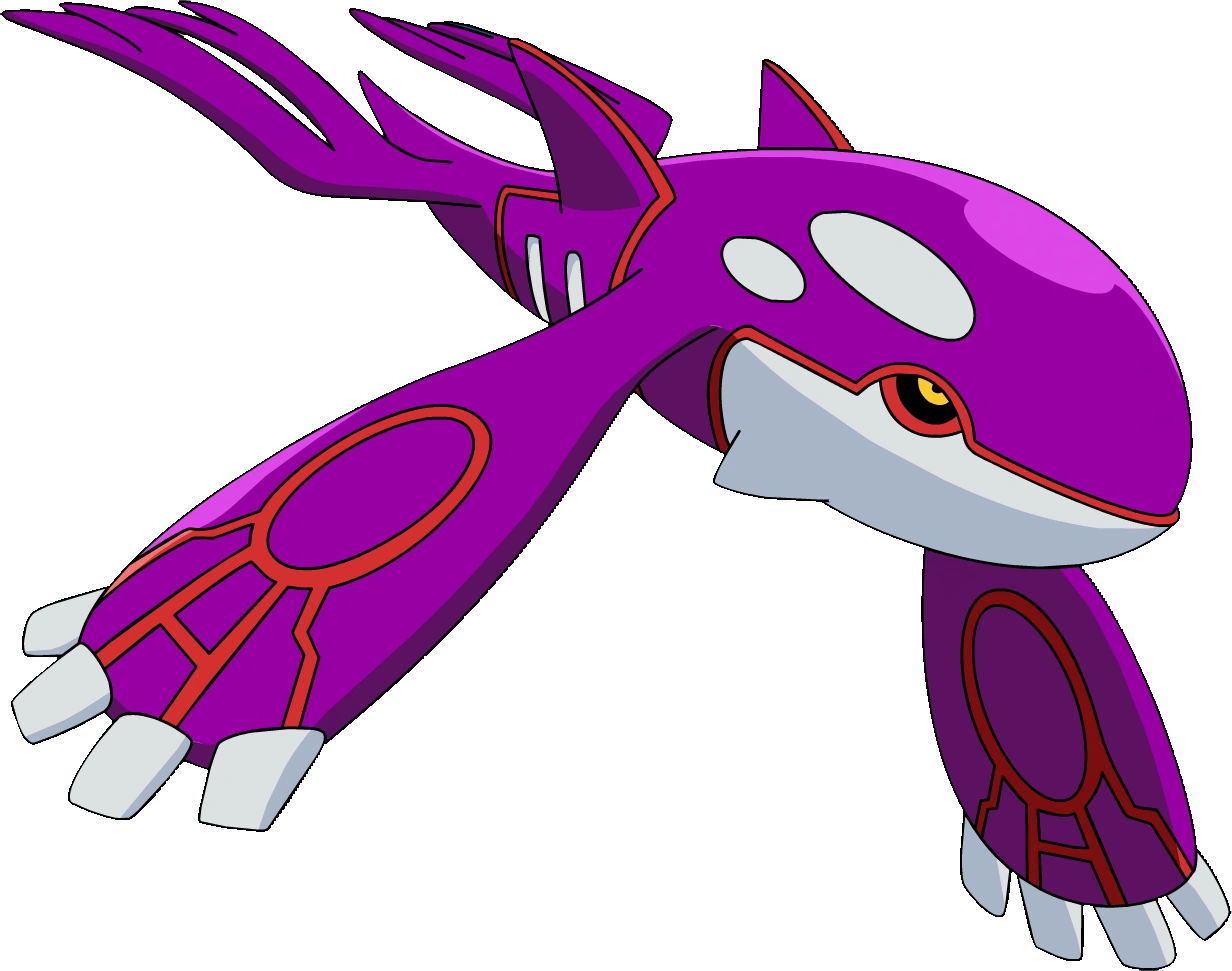
\includegraphics[width=\linewidth,keepaspectratio]{images/kyogre.png}
\section{Crowned forms\label{sec:crowned}}
\nopagecolor
Crowning is a reversible, persistent evolution available to Zacian and Zamazenta
 so long as they know the charged attack Iron Head.
Upon coronation, stats are modified, and Iron Head is replaced with Behemoth Blade (Zacian)
  or Behemoth Bash (Zamazenta).
This new attack cannot be changed with even an Elite Charged TM\@.
A Crowned form can fight in Max Battles (though it \textit{cannot} be left at Power Stops), with Behemoth Blade/Bash as its Max Attack.
This Max Attack follows the same rules for leveling, power, and use as any other Dynamax attack.
Crowning consumes 1,000 Crown Energy, but once a Pokémon has been crowned,
  that Pokémon can freely change between the base and crowned
  forms\footnote{I'm not sure why one would uncrown. Perhaps to change charged attacks?
    Eliminate Steel typing? Most likely to trade the Pokémon.}, even if traded.
Crowned Shield Zamazenta can stack four Guards rather than the typical three.
If it has Max Guard unlocked, it starts Max Battles with one Guard already in place.

\input{out/crowned}

\section{Fused forms\label{sec:fusion}}
Certain Pokémon can be reversibly fused, yielding a new form.
The fusion process requires 1,000 units of Fusion Energy particular to the output\footnote{They all kinda sound like Mountain Dew flavors.},
 and 30 Candy of each input species (\autoref{table:fusion}).
There is no cost to undo the fusion, but subsequent fusions cost the same amount as the initial fusion.
Any powering up performed on the fused form will apply only to the primary
  Pokémon if the fusion is undone, the fused form's IV is taken from the primary Pokémon,
  and fusion replaces the first charged attack of the primary Pokémon (\autoref{table:fusionattacks}).
\begin{table}
\centering
\begin{tabular}{llll}
Primary & Secondary & Energy & Output\\
\Midrule
Kyurem & Zekrom & Volt & Black Kyurem \\
Kyurem & Reshiram & Blaze & White Kyurem \\
Necrozma & Solgaleo & Solar & Dusk Mane Necrozma \\
Necrozma & Lunala & Lunar & Dawn Wings Necrozma \\
\end{tabular}
\caption{Fusion paths\label{table:fusion}}
\end{table}
\begin{table}
\centering
\begin{tabular}{ll}
Fused form & Attack\\
\Midrule
Black Kyurem & Freeze Shock \\
White Kyurem & Ice Burn\\
Dusk Mane Necrozma & Sunsteel Strike\\
Dawn Wings Necrozma & Moongeist Beam\\
\end{tabular}
\caption{Special fused attacks\label{table:fusionattacks}}
\end{table}

\input{out/fused}
